\chapter{Implementation}

\section{Installing gateways in Furtwangen}

\ac{TTNM} already had a number of data points for existing \ac{LoRaWAN} gateways in the Furtwangen area.
However, to make a good geolocation prediction for a \ac{LoRaWAN} node, it is necessary to have at least three gateways in range of the node.

Since, at the beginning of this thesis, there were only two gateways installed in the vicinity of Furtwangen, the first step was to research, order and then install additional gateways in the city.

Some gateways that were used in this thesis were ones that were already in the possession of the \ac{HFU}.
Such was the case for the \emph{Dragino LG308 / LG308N} indoor gateways as well as a \emph{RAK7258} indoor gateway.

Additionally, for development purposes, a \emph{Dragino PG1301} gateway was also used.
The PG1301 is designed to be used with a Raspberry Pi and mounts on top of it in typical Raspberry Pi shield fashion.

\subsection{Researching gateways}

Two MikroTik wAP LR8 kit gateways were purchased for the thesis.
They were chosen after recommendation by a member of the \ac{HSN-TTN} team~\cite{hochschwarzwald_smart_net_-_thethingsnetwork_eingesetzte_nodate}.
The MikroTik wAP LR8 kit was a compelling offer due to its low price and the fact that it comes with MikroTik's \emph{RouterOS}, a well-established GUI for configuring networking devices~\cite{mikrotik_mikrotik_nodate}.
A picture of this gateway can be seen in \cref{pic:mikrotik-lr8-kit-gateway}.
The antenna used with the MikroTik wAP LR8 kit is also from MikroTik, which is a 6.5 dBi antenna which can be seen in \cref{pic:mikrotik-antenna-c-building}.

The other gateway that was purchased for the thesis was a \emph{Dragino DLOS8N} outdoor gateway.
This gateway was chosen because of difficulties in ordering the second MikroTik wAP LR8 kit.
It was available right away at the time of ordering and was thus chosen as a short-term replacement.
It was used even after the second LR8 arrived as the user interface is identical to the one used in the Dragino LG308 gateway which made it easy to set up.
The DLOS8N also has a case that is weatherproof and made for outdoor use, making it similarly suitable as the LR8.

\subsection{Locations}

% TODO: Add map with Gateway locations (later)

Multiple locations proved themselves to be worth considering when it came to installing new \ac{LoRaWAN} gateways in Furtwangen.
In the following sections, the chosen locations are described and evaluated.

\subsubsection{\ac{HFU} B and C building}

The first antenna and gateway installed was a Dragino LG308 connected to a MikroTik antenna on top of the \ac{HFU} C building as seen in \cref{pic:mikrotik-antenna-c-building}.
While not as high in altitude as the \ac{GHB} building, it was thought to still be a good location to receive signals from the surrounding area.
The roof of the C building is located in the center of the valley Furtwangen is situated in.

Another gateway with antenna was deployed on top of the B building as there already was ample infrastructure available.
Additionally, this roof was two stories higher than the C building roof, making it a good location for a gateway as well.
A Dragino DLOS8N gateway was used here because of its ability to easily be powered by \ac{PoE}.

\subsubsection{\acf{GHB} student dormitory}

The \ac{GHB} is a popular student dormitory located on the Großhausberg mountainside in Furtwangen~\cite{ghb_netadmins_student_2023}.
Its exposed location and the fact that it is among the highest buildings in the city makes it a good location for putting up a \ac{LoRaWAN} gateway.

The network infrastructure of both the \ac{GHB} and the \ac{ASH} are managed by the ``\ac{GHB} NetAdmins'' who are students of \ac{HFU}.
With their help, it was possible to install antennas on the roofs of the \ac{GHB} and \ac{ASH} student dormitories.

\begin{figure}
    \centering
    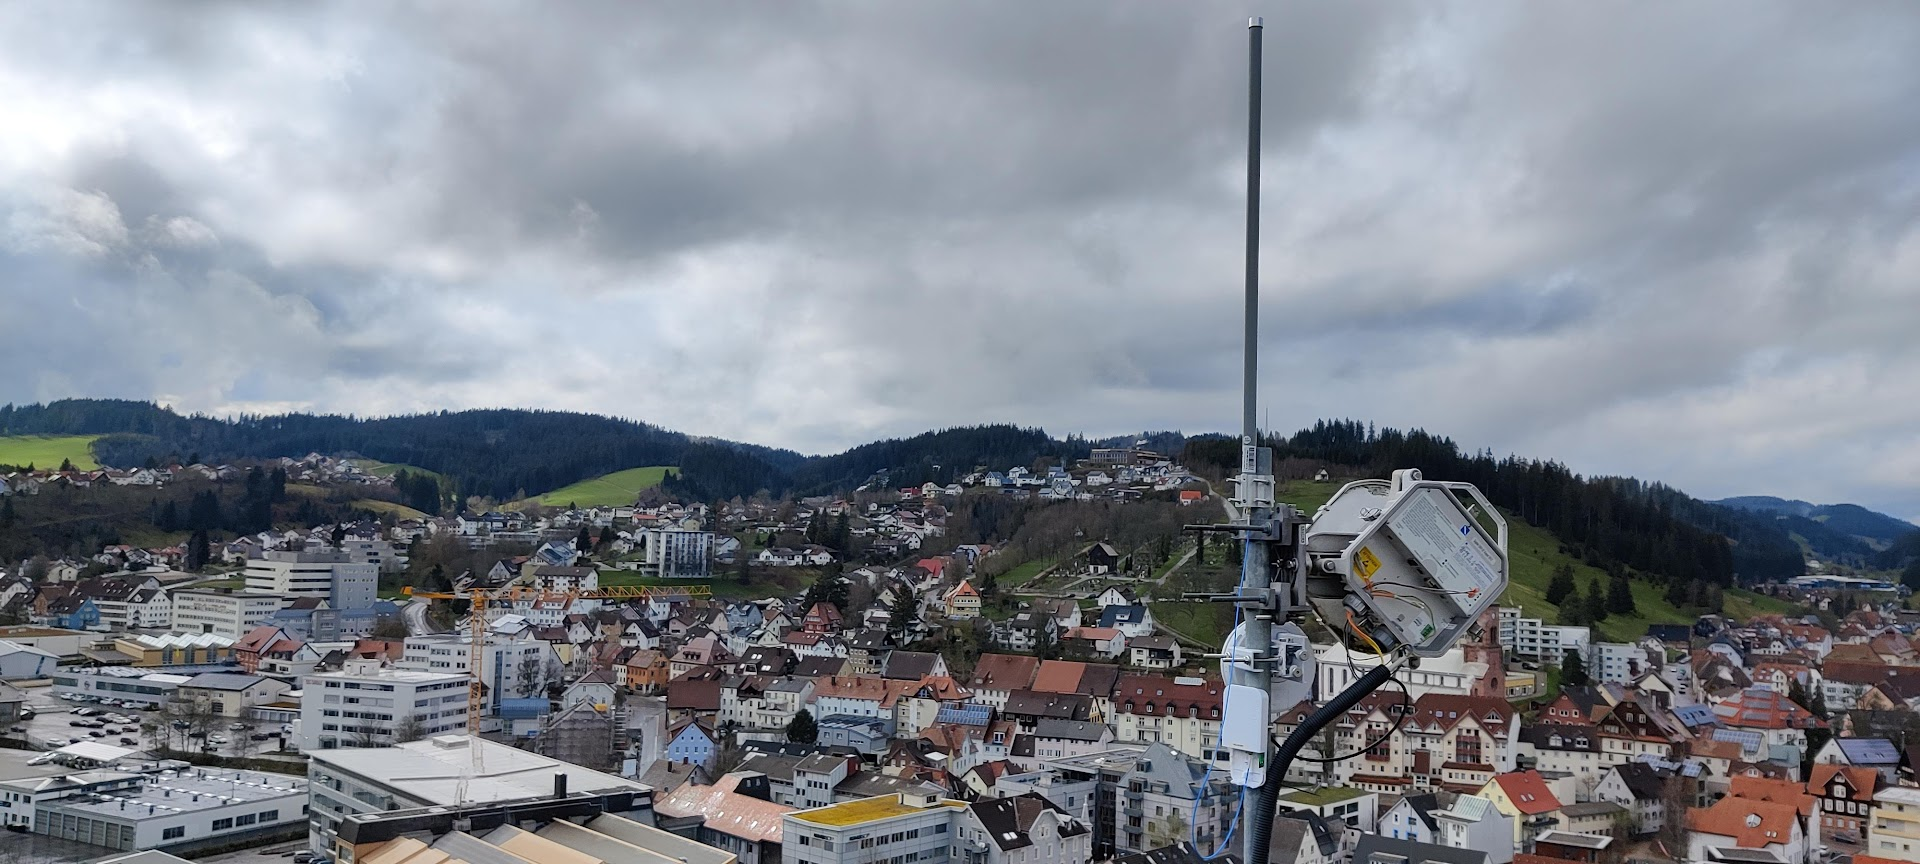
\includegraphics[width=1\textwidth]{pictures/hardware/gateway-deployment/lr8_ghb_installation.jpg}
    \caption{Installed MikroTik LR8 wAP gateway with antenna on the \ac{GHB} student dormitory\label{pic:mikrotik-gateway-ghb-installation}}
\end{figure}

\Cref{pic:mikrotik-gateway-ghb-installation} shows the installed MikroTik wAP LR8 kit gateway on the roof of the \ac{GHB} student dormitory.
Again, \ac{PoE} was used to power the gateway since only one cable needed to be put through the existing cable duct.

\subsubsection{\acf{ASH}}

The \ac{ASH} is a former student dormitory located in the Furtwangen city area which is currently used as housing for refugees from the ongoing war between Ukraine and Russia.
It is located on a hillside in the city area and is thus a good location for a \ac{LoRaWAN} gateway.
Its network infrastructure is also managed by the ``\ac{GHB} NetAdmins'', which made getting it connected to \ac{HFU} network infrastructure painless with their forthcoming support.

\begin{figure}
    \centering
    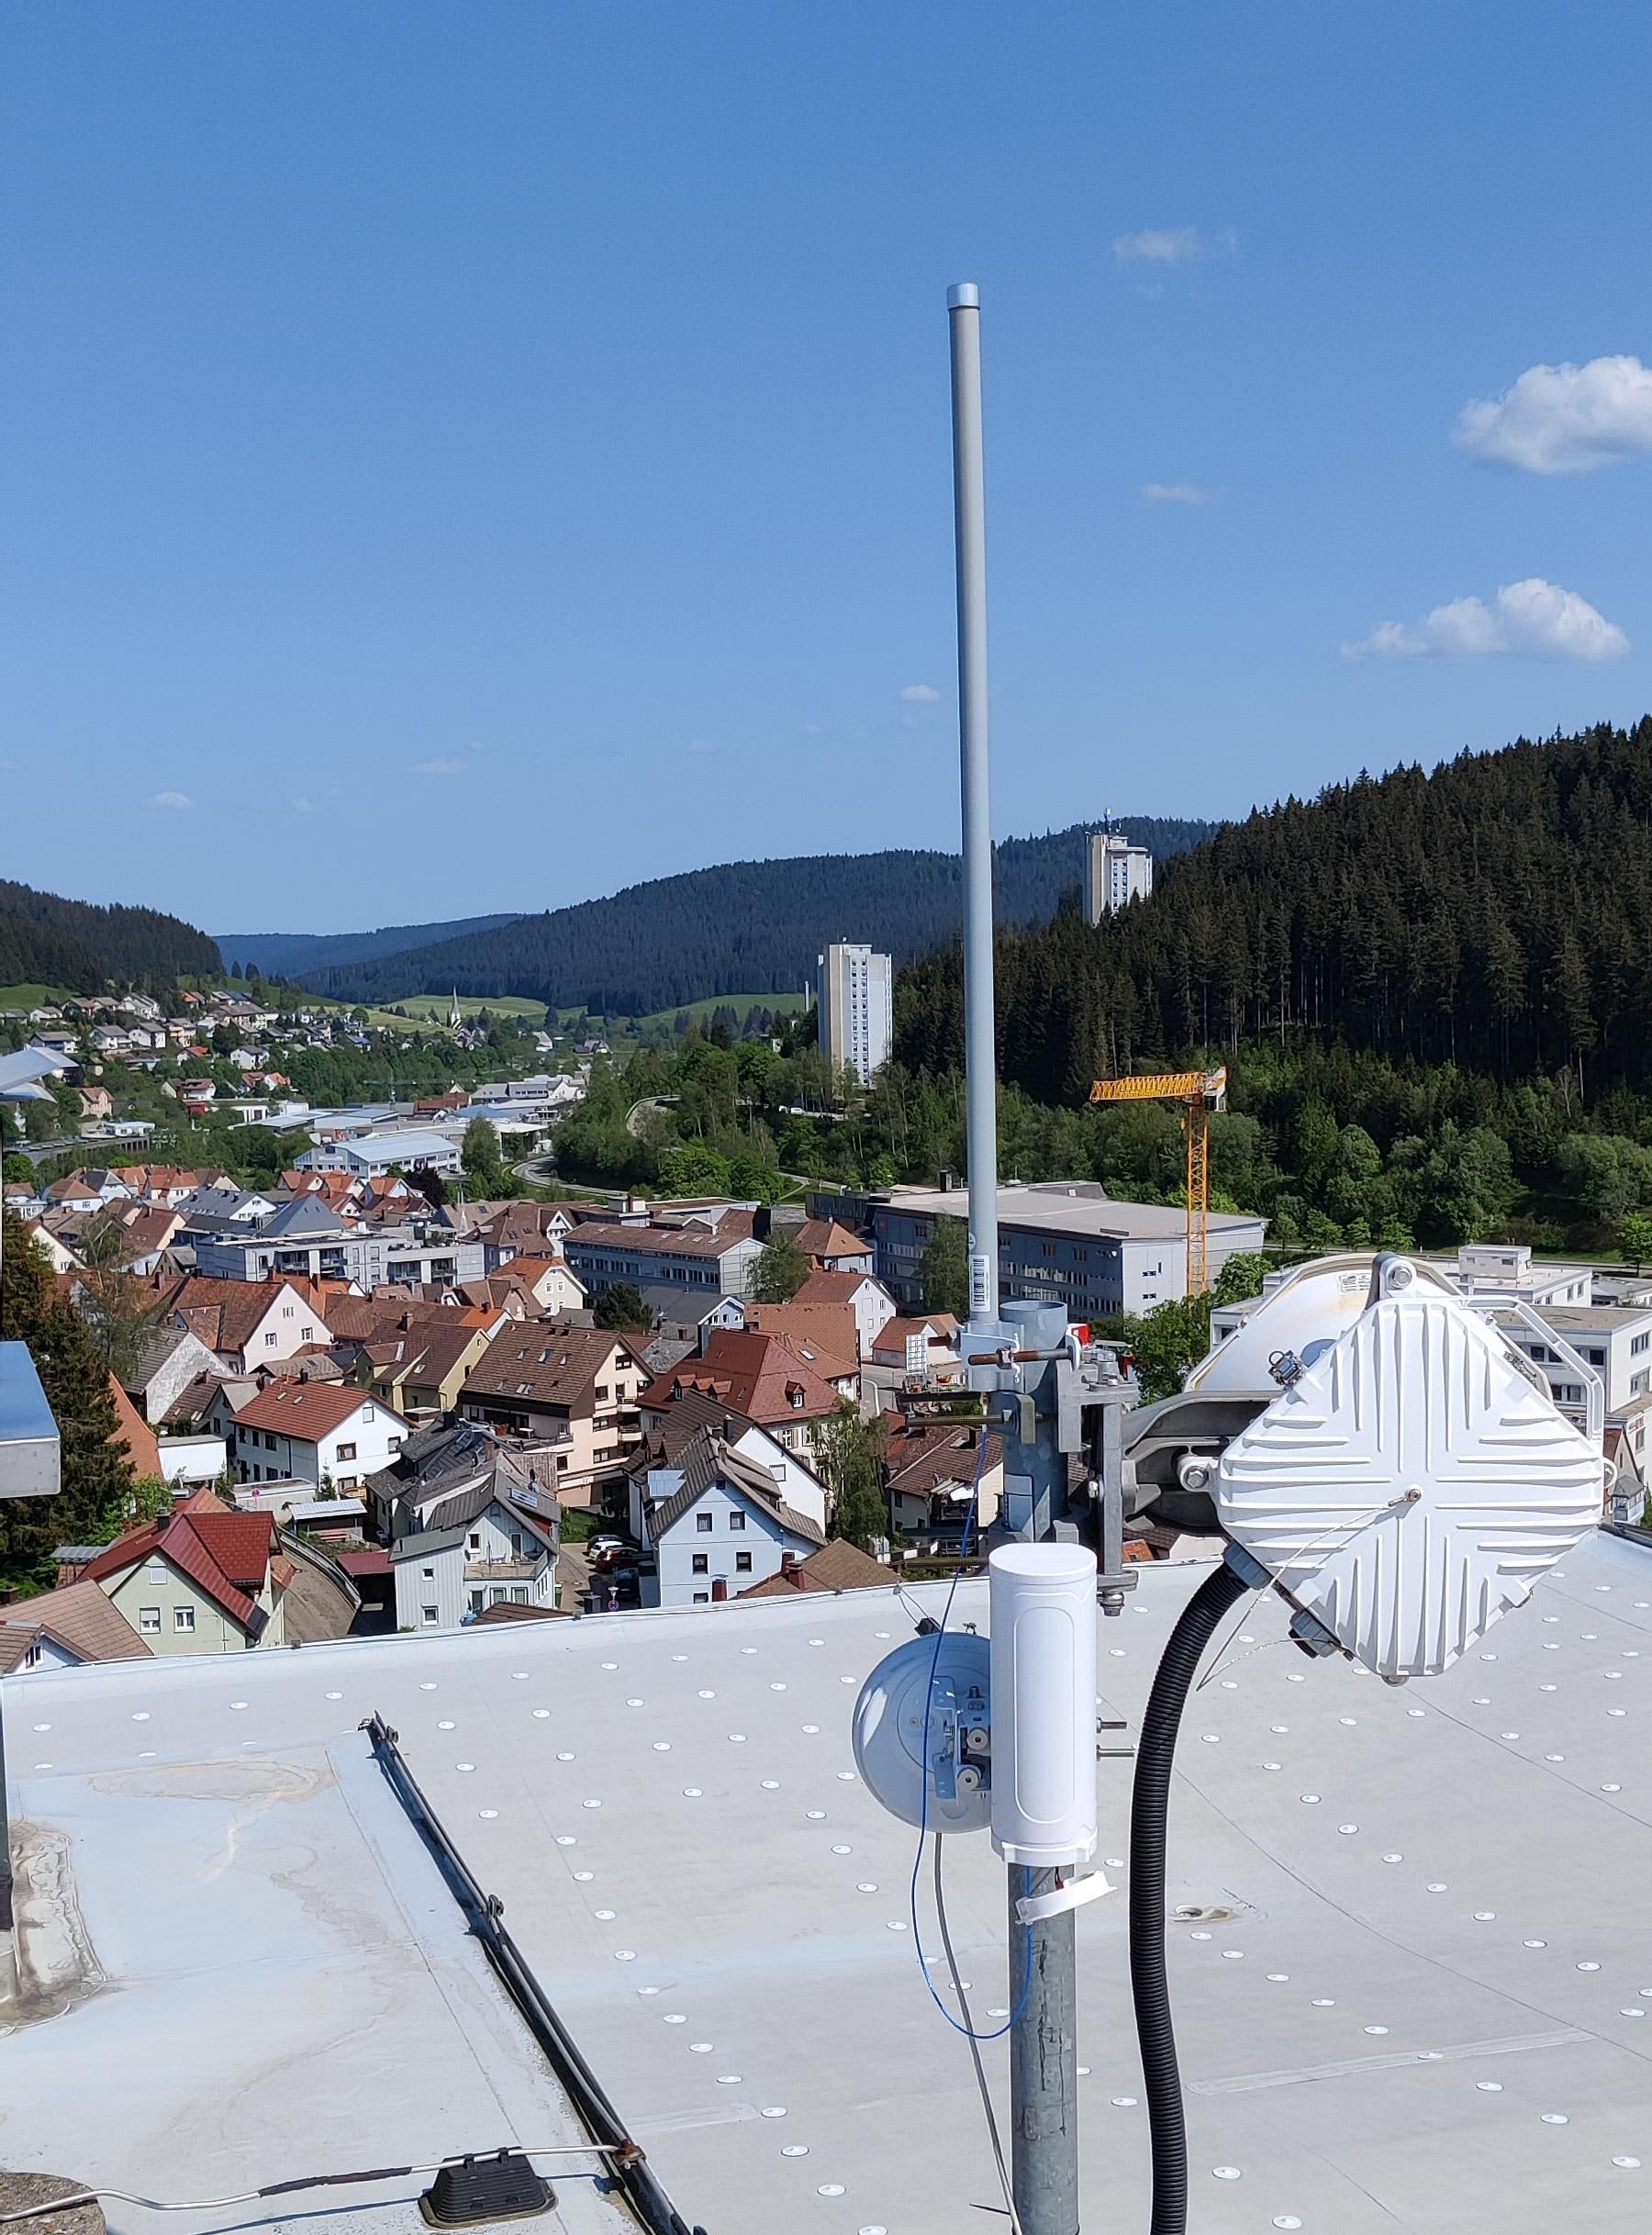
\includegraphics[width=0.5\textwidth]{pictures/hardware/gateway-deployment/gateway_ash.jpg}
    \caption{Installed Dragino DLOS8N gateway with antenna on the \acf{ASH}\label{pic:dragino-gateway-ash}}
\end{figure}

\Cref{pic:dragino-gateway-ash} shows the installed Dragino DLOS8N gateway on the roof of the \ac{ASH} student dormitory.
This gateway is also powered by \ac{PoE}.
The ``\ac{GHB} NetAdmins'' already had a network switch with \ac{PoE} capabilities installed in the \ac{ASH} which made it easy to power the gateway.

\subsubsection{\emph{DL0FIS} amateur radio club station (Neueck, Gütenbach)}

\section{Collecting additional \acf{TTNM} data in the Furtwangen area}\label{sec:collecting-additional-ttnm-data}

In order to have more data to work with as far as geolocation calculations are concerned, there was a need to collect more \ac{LoRaWAN}, \ac{RSSI} and \ac{GPS} data that could be synthesized.
This data was especially important for doing geolocation calculations via fingerprinting.

This was done by using \ac{LoRaWAN} nodes that were equipped with \ac{GPS} modules and then moving them around the city of Furtwangen.

\subsection{Used \acs{LoRa} nodes}

In this chapter, the \ac{LoRa} nodes used for collecting \ac{GPS} data for \ac{TTNM} are described are briefly evaluated.

\subsubsection{ELV LW experimental platform}

\begin{figure}
    \centering
    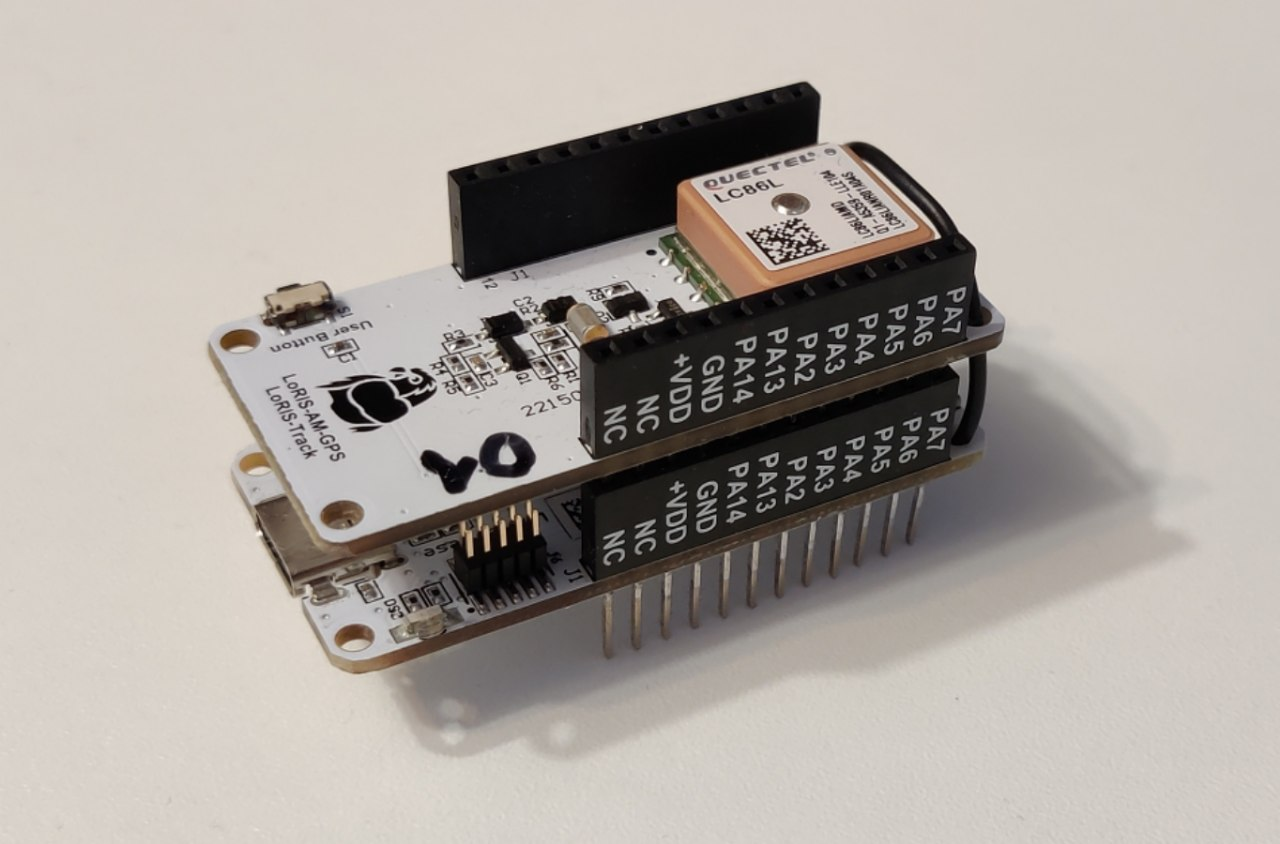
\includegraphics[width=0.5\textwidth]{pictures/hardware/gps-nodes/loris_bare.jpg}
    \caption{ELV-AM-GPS \ac{LoRaWAN} node on top of the LoRIS base\label{pic:loris-node-bare}}
\end{figure}

The ELV LW experimental platform was the \ac{LoRaWAN} node out of the ones used during this thesis that worked best out of the box as far as overall usability is concerned\cite{elv_elektronik_ag_elv-lw-base_2023}.
The ELV LW experimental platform consists of a base module called ELV-BM-TRX1 and a number of different sensor modules that can be stacked on top of it as seen in \cref{pic:loris-node-bare}.
It has a USB-C port, which made powering the tracker with an external power bank simple.

Little had to be done in order to begin using the base with the additional \ac{GPS} module ELV-AM-GPS~\cite{elv_elektronik_ag_elv-track_2022}.
Flashing the firmware using a tool provided by the manufacturer was the first step.
Additionally, the \ac{OTAA} credentials provided in the box of the base LoRIS module had to be entered into \ac{TTN}.

\begin{figure}
    \centering
    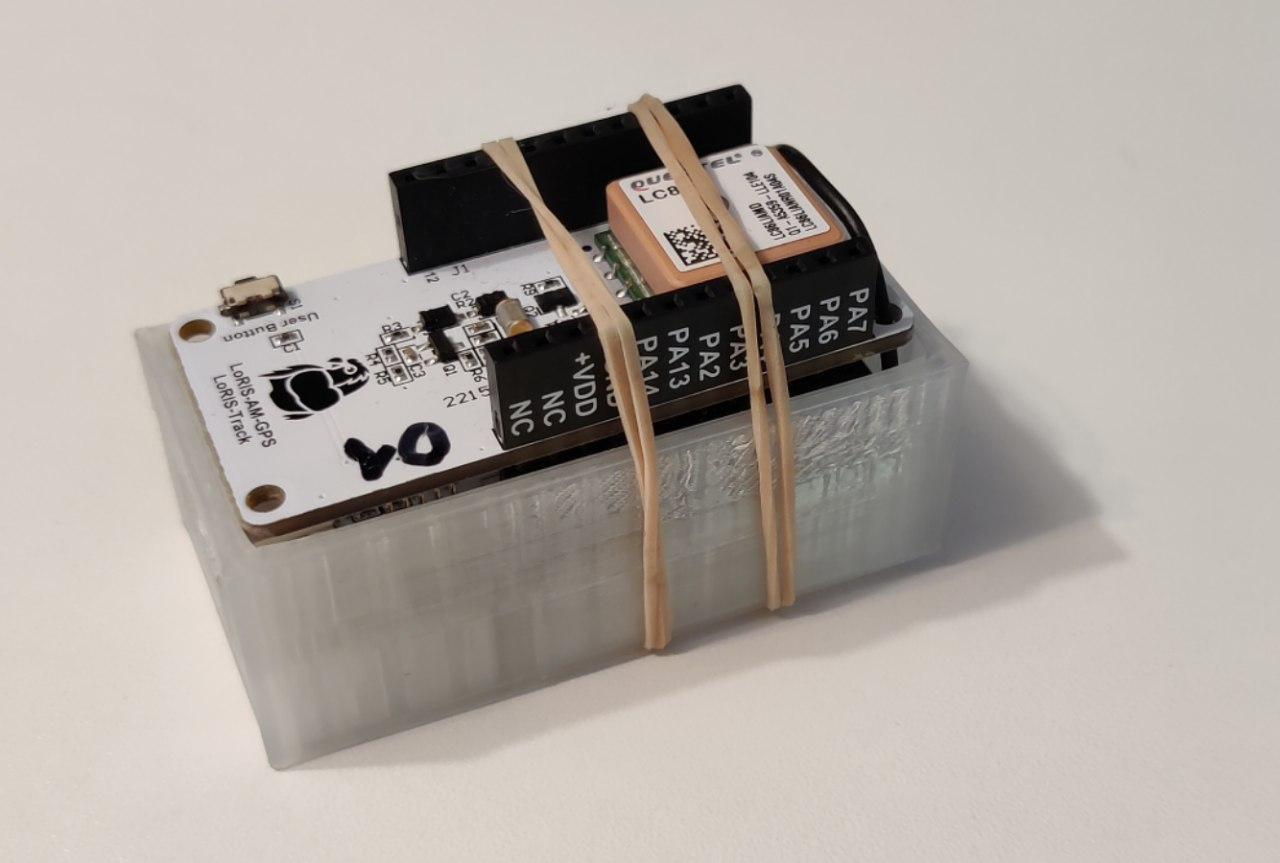
\includegraphics[width=0.5\textwidth]{pictures/hardware/gps-nodes/loris_with_case.jpg}
    \caption{ELV-AM-GPS \ac{LoRaWAN} node in self-designed 3D printed case\label{pic:loris-node-with-case}}
\end{figure}

To make the board a little more robust, a 3D printed case was designed in Fusion 360 and printed as can be seen in~\cref{pic:loris-node-with-case}.

\subsubsection{ELV \acs{GPS} Tracker}

\begin{figure}
    \centering
    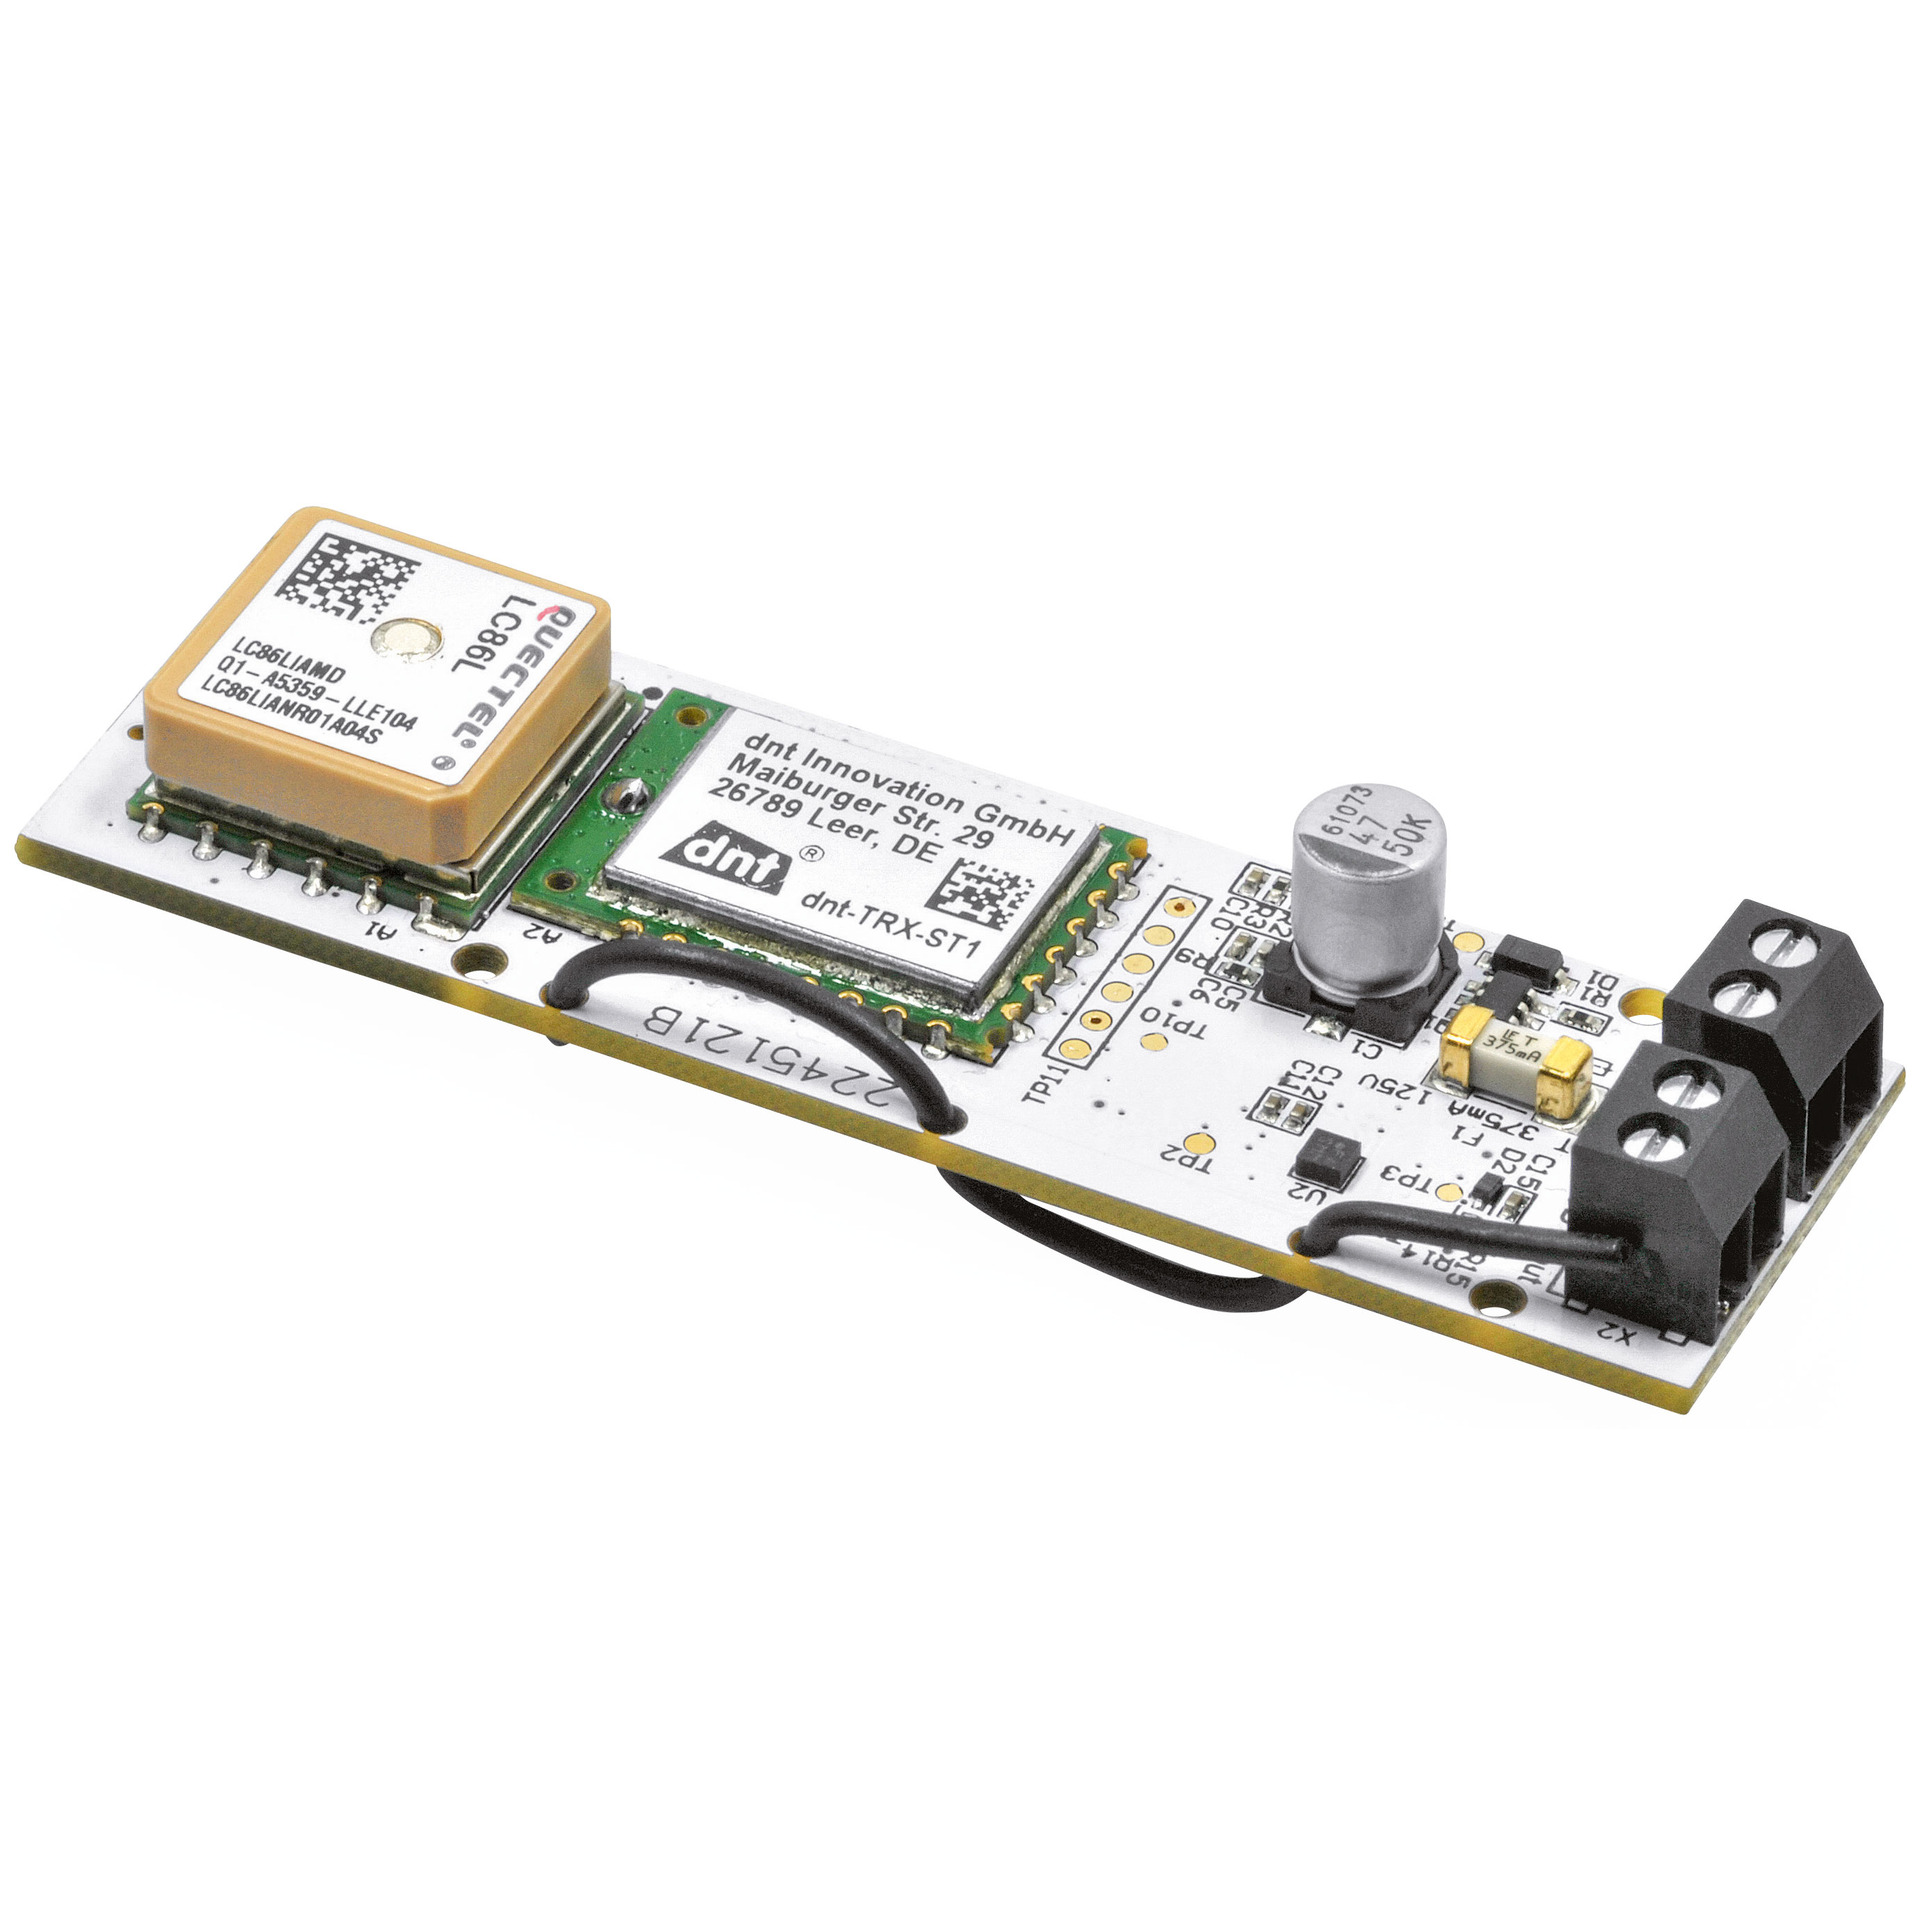
\includegraphics[width=0.6\textwidth]{pictures/hardware/gps-nodes/ELV-LW-GPS1.jpg}
    \caption{ELV-LW-GPS1 \ac{LoRaWAN} node~\protect\cite{elv_elektronik_ag_elv_2023}}
\end{figure}

The ELV-LW-GPS1 is another \ac{LoRaWAN} node that is designed to be used as a \ac{GPS} tracker.
Its specialty is that it takes a power source that can range from 5 to 40 volts.
This fact makes it flexible in terms of power supply and makes it possible to use it, for example, with a car battery that usually has a voltage of 12 volts.

Finding a power source to be able to use it for this thesis was a challenge.
While it can be powered by a 9V battery, those usually have a low capacity and are not rechargeable.

% TODO how was this solved?

\subsubsection{Heltec HTCC-AB02S}

% didn't work well enough without additional GPS antenna
% screen is pretty nice, though

% TODO

\subsubsection{dnt-LW-ATS}

% TODO
\begin{figure}
    \centering
    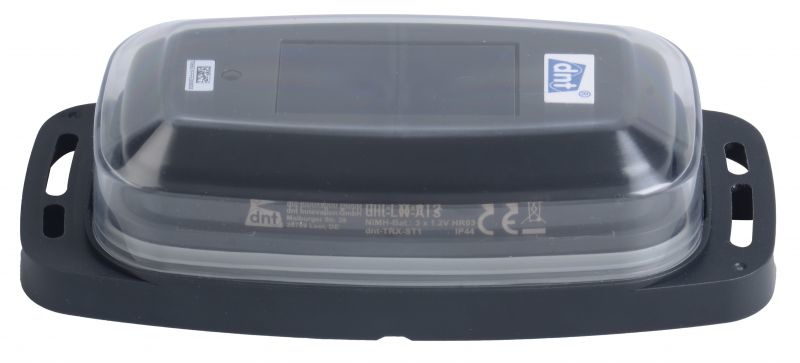
\includegraphics[width=0.6\textwidth]{pictures/hardware/gps-nodes/dnt-LW-ATS.jpg}
    \caption{dnt-LW-ATS \ac{LoRaWAN} node~\protect\cite{dnt_gmbh_dnt_nodate}}
\end{figure}

At first glance, this was the most promising \ac{LoRa} node for the task at hand.
It has a built-in \ac{GPS} module as well as a weatherproof, IP44 rated exterior case and a solar panel for charging the internal battery.

However, the node was challenging to set up and operate.
The device offers a \emph{motion based cyclic} mode in which, during physical movement, the node sends its \ac{GPS} coordinates to \ac{TTN} every few seconds.
This, however, did not work in practice and the node would only send its coordinates very irregularly, if at all.
The documentation was not very helpful with finding the root cause and the manufacturer could only offer to replace the hardware.

\subsection{\acl{TTNM} heatmap view before additional data collection}

\begin{figure}
    \centering
    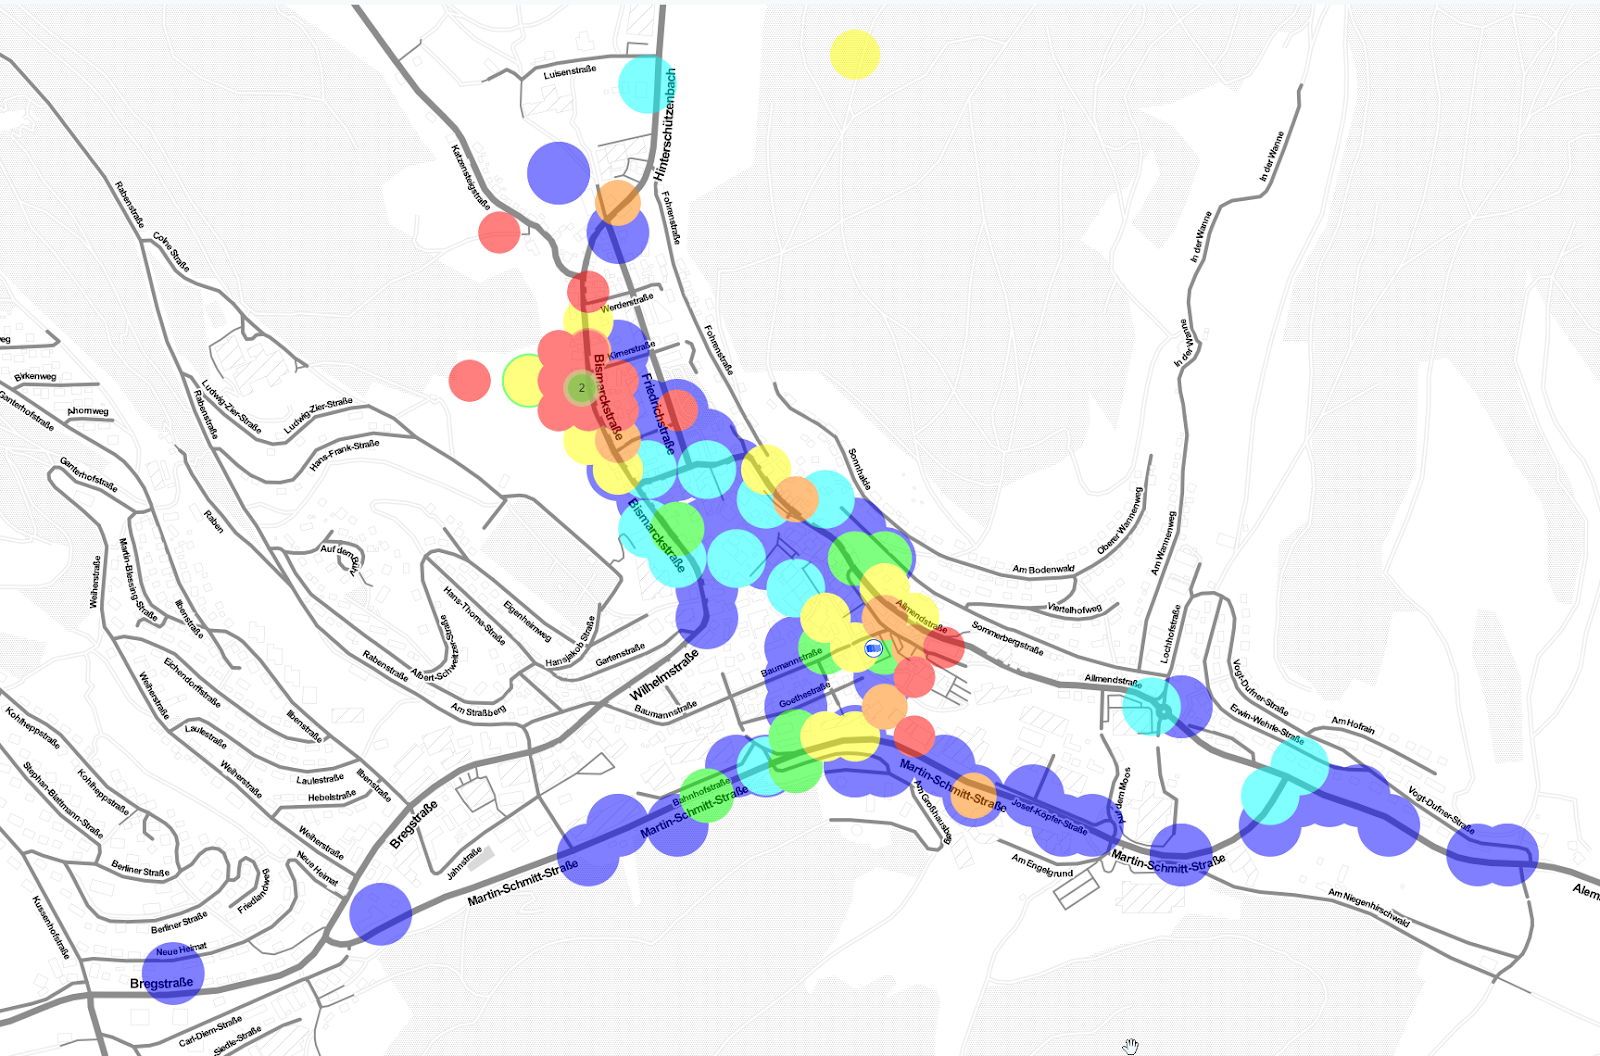
\includegraphics[width=0.6\textwidth]{pictures/ttn-mapper/ttnmapper_heatmap_before.png}
    \caption{\ac{TTNM} heatmap view before additional data collection during this thesis\label{pic:ttnm-before-data-collection}}
\end{figure}

\Cref{pic:ttnm-before-data-collection} shows the \ac{TTNM} heatmap view before additional data collection during this thesis.
As mentioned in \cref{sec:collecting-additional-ttnm-data}, additional data needed to be collected in order to be able to create better fingerprinting results.
\Cref{sec:ttm_heatmap_after} shows the heatmap view after additional data collection.

\section{Used development tools}

% TODO: is this necessary?

\subsection{Visual Studio Code}

\subsubsection{Extensions}

\section{Program structure: \acf{TTNL}}\label{section:ttnl}

The programmatic implementation of this thesis was called \acf{TTNL} and split into two parts: the backend and the frontend.

\subsection{Overview}

% TODO add diagram of program structure

% TODO mention the extensive usage of docker and docker-compose to enable easy deployment of the application

\subsection{Database}

% TODO add ER diagram of database

\subsection{Used technologies --- Backend}

This chapter describes the technologies used in the backend part of the \ac{TTNL} web application.
The chosen stack uses Express.js with \ac{TS} as the programming language, PostGIS as the database system as well as the Prisma \ac{ORM} to connect to the \ac{DB}.
These services are designed to be running in Docker containers and are orchestrated using Docker Compose.

\subsubsection{\acf{JS} / \acf{TS}}

\ac{JS} is an interpreted, \ac{JIT} compiled programming language that was designed for and is mostly used in web browsers to add interactivity to websites~\cite{mdn_javascript_2023}.
However, it can also be used outside a browser, for example, to create server applications as is explained in \cref{sec:nodejs}.

\ac{TS}, on the other hand, is a superset of \ac{JS} that adds static type checking to the language~\cite{microsoft_javascript_nodate}.
This means that the developer has to specify the types of variables and function parameters, which are then checked by the compiler.
Assigning the wrong type to a variable or passing the wrong type to a function then triggers compile-time error instead of a runtime error.

\begin{lstlisting}[language=TypeScript, float, caption={Example of type checking in \ac{TS}}, label={lst:example-ts-type-checking}]
const user = {
    firstName: "Teysa",
    lastName: "Karlov",
    role: "Guildmaster",
}
    
console.log(user.name)
\end{lstlisting}

\Cref{lst:example-ts-type-checking} shows an example of how \ac{TS} can help prevent runtime errors.
The \ac{TS} compiler would show the message \lstinline|Property `name' does not exist on type { firstName: string; lastName: string; role: string; } | since \lstinline{name} is not a property of the \lstinline{user} object.

\subsubsection{Node.js}\label{sec:nodejs}

Node.js is a \ac{JS} runtime environment that allows for the execution of \ac{JS} code outside a web browser~\cite{noauthor_nodejs_nodate}.
It uses the \emph{V8} \ac{JS} engine, which is also used in the Google Chrome web browser~\cite{noauthor_v8_nodate}.
Its main benefit is being able to use a single language for both frontend and backend development --- \ac{JS}, or, in this case, \ac{TS}.

Node.js is available as a Docker image, which makes it easy to use in the Docker Compose setup used in this thesis~\cite{docker_inc_node_2023}.

\subsubsection{Express.js}

Express.js is a ``fast, unopinionated, minimalist web framework for Node.js''~\cite{noauthor_express_nodate}.
``Unopinionated'' means that it does not enforce any specific way of implementing a web application and instead focuses on the premise ``configuration over convention'', leaving the developer to decide how to implement the specifics of the application~\cite{mardan_pro_2014}.

It was used in this thesis as a means to implement the backend part of the \ac{TTNL} web application.
Express.js allows for the creation of \ac{REST} \ac{API} endpoints that can be used by the frontend or by other applications.

\begin{lstlisting}[language=TypeScript, float, caption={Example of an Express.js \ac{API} endpoint}, label={lst:express-api-endpoint}]
router.get('/', async (request: Request, response: Response) => {
    const numberOfDeviceSubscriptions = await GetterFunctions.getAmountOfDeviceSubscriptions();
    response.send({
        message: `Hello from ttn-locator-backend!\nCurrent amount of Device subscriptions: ${numberOfDeviceSubscriptions}`,
    });
});
\end{lstlisting}

\Cref{lst:express-api-endpoint} is an example of an Express.js \ac{API} endpoint that returns a simple message along with the current amount of device subscriptions~\cite{noauthor_express_nodate-1}.
Express also allows for the creation of more complex endpoints that can, for example, return data from a database.
Additionally, routes for different parts of requested data can be defined and put into separate files, making the code more navigable.

\subsubsection{PostgreSQL / PostGIS}

PostgreSQL is an open-source \ac{RDBMS} that is available for a variety of operating systems~\cite{postgresql_global_development_group_postgresql_2023}.
It is among the most popular database management systems worldwide~\cite{db-engines_most_2023}.

In this thesis, for \ac{TTNL}, PostgreSQL was used as the database management system because of its popularity, its possibility to be used with the \ac{ORM} Prisma as well as PostGIS.\
PostGIS is an extension for PostgreSQL that adds support for geographic objects and allows for geographic queries~\cite{postgis_psc__osgeo_postgis_2023}.

\begin{lstlisting}[language=SQL, float, caption={Example of a PostGIS query to calculate the distance between two geolocation points in meters}, label={lst:postgis-example-distance}]
SELECT ST_DistanceSphere(
    ST_MakePoint(8.2047, 48.0502), -- Furtwangen
    ST_MakePoint(7.85222, 47.9959) -- Freiburg
);

Result => 26900.55162337
\end{lstlisting}

\Cref{lst:postgis-example-distance} shows an example of a PostGIS query that calculates the distance in meters between two points on the earth's surface~\cite{noauthor_st_distancesphere_nodate}.

PostGIS is also available as a Docker image, making it easy to deploy in the given docker compose setup~\cite{docker_inc_postgispostgis_2023}.

\subsubsection{Prisma}

Prisma is an \ac{ORM} that can be used with a variety of database management systems, including PostgreSQL~\cite{prisma_data_inc_prisma_2023}.
\acp{ORM} allow for the creation of database queries using the programming language of the application instead of using the database's query language, which would be \ac{SQL} in the case of PostgreSQL.\
Instead, Prisma allows for the creation of queries using \ac{TS}.
Prisma also lets the developer define a database schema and can generate migrations to generate the database tables from that schema.

\begin{lstlisting}[float, caption={Example of a Prisma schema}, label={lst:prisma-schema-example}]
model User {
    id    Int     @id @default(autoincrement())
    posts Post[]
}
    
model Post {
    id       Int   @id @default(autoincrement())
    author   User? @relation(fields: [authorId], references: [id])
    authorId Int?
}
\end{lstlisting}

\Cref{lst:prisma-schema-example} shows an example of a Prisma schema that defines two database tables, \lstinline{User} and \lstinline{Post}, and their relationship: A User can have many Posts.

While Prisma enables the developer to write type safe database queries using \ac{TS}, it does not support all possible queries (yet).
Some advanced queries, such as the one shown in \cref{lst:postgis-example-distance}, had to be written by hand using \ac{SQL} and executed using Prisma's \lstinline|$executeRaw| method.

% TODO: this maybe should be in the conclusion section?
There were several such cases in this thesis, which is why it might have been more suitable to not use Prisma at all and instead use \ac{SQL} in a more direct way.
However, Prismas ability to generate migrations from a schema and its type safety were still useful features that made it worth using.
Prisma's schema file also acts as indirect documentation of the database structure, which is useful for other developers that might want to contribute to the project.

% TODO also add my own complete prisma schema?

\subsubsection{Vitest}

Vitest is a testing framework for \ac{JS} and \ac{TS}~\cite{vitest_team_vitest_2023}.
It was used in this thesis to write unit as well as intergration tests for the backend part of the \ac{TTNL} web application.
Vitest uses a syntax that is similar to Chai/Jest, which is a popular syntax for writing tests in \ac{JS} and \ac{TS}~\cite{vitest_team_vitest_2023-1}.

\subsection{Used technologies --- Frontend}

\subsubsection{Vue.js}

Vue.js is a \ac{JS} framework for building reactive user interfaces~\cite{evan_you_vuejs_2023}.
It was used in this thesis as a means to implement the frontend of the \ac{TTNL} web application.
Vue can also use \ac{TS} as a programming language, which was used in this thesis for making the code more robust and easier to maintain due to its type safety.

Vue.js was chosen because of the author's previous experience with it and because of its ease of use and quick development time.
It also offers many plugins and libraries that can be used to extend its functionality as well as a large community that can be consulted for help.

\subsubsection{Vuetify}

Vuetify is a \ac{UI} framework for Vue.js that provides Vue components that are based on Google's Material Design guidelines~\cite{vuetify_vuetify_2023}~\cite{google_llc_material_nodate}.
In this thesis, Vuetify was used as a modern looking \ac{UI} framework for the frontend of the \ac{TTNL} web application.
Its usage as import-able predefined Vue components also allowed for a quick and easy implementation of the frontend.

\begin{figure}
    \centering
    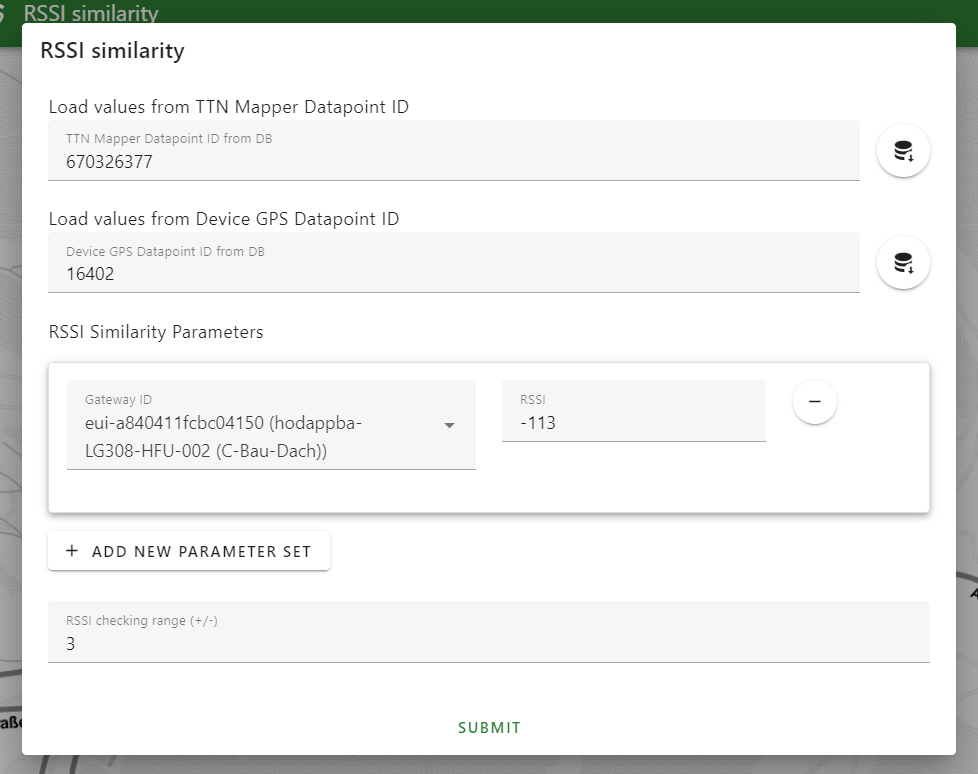
\includegraphics[width=0.8\textwidth]{pictures/ttn-locator/frontend/vuetify-form-example.png}
    \caption{An example of a form created using Vuetify components\label{fig:vuetify-form-example}}
\end{figure}

\Cref{fig:vuetify-form-example} shows an example of a form created using Vuetify components in the \ac{TTNL} frontend.
It uses several of Vuetify's components to enable the user to enter \ac{RSSI} values for several gateways for localization purposes.

\subsubsection{Leaflet}

Leaflet is a \ac{JS} library for displaying interactive maps in the browser~\cite{volodymyr_agafonkin_leaflet_2023}.
It currently has around 800,000 weekly downloads on the npm package repository~\cite{npm_leaflet_2023}.
It was used in this thesis to display the map on the frontend of the \ac{TTNL} web application.
Leaflets widespread use and large community made it a good choice for this purpose since there are many examples and tutorials available online.

To make Leaflet work with Vue.js, the \emph{vue2-leaflet} plugin was used~\cite{noauthor_vue_nodate}.
It wraps Leaflet's functionality into Vue components and provides reactive bindings for Leaflet's properties and map data.

\subsubsection{GeoJSON}

GeoJSON is a format used for representing geographical data using the popular \ac{JSON} format~\cite{butler_geojson_2016}.
This format was used in this thesis as a means to standardify the data format used for representing geographical data as well as its communication between client and server.

\begin{lstlisting}[language=JSON, float, caption={Example of a GeoJSON that represents a rectangle above the furtwangen city center}, label={lst:geojson-example}]
{
    "type": "FeatureCollection",
    "features": [
        {
            "type": "Feature",
            "properties": {},
            "geometry": {
                "coordinates": [
                    [
                        [8.2032444080252, 48.05293370858834],
                        [8.2032444080252, 48.04823334925436],
                        [8.20949460707348, 48.04823334925436],
                        [8.20949460707348, 48.05293370858834],
                        [8.2032444080252, 48.05293370858834]
                    ]
                ],
                "type": "Polygon"
            }
        }
    ]
}  
\end{lstlisting}

\Cref{lst:geojson-example} shows an example of a GeoJSON object.

\subsection{Consolidating \acl{TTNM} data into the \acl{TTNL} database}

To be able to perform more advanced queries on the data, it needed to be, partly, transferred \ac{TTNL} database.
Since, for the scope of this thesis, only devices that captured data near the Furtwangen area were of interest, only data from those devices was transferred.
This is because fingerprinting on a larger or even global scale would likely result in the need for a much bigger, maybe even distributed \ac{RDBMS}.
However, the \ac{TTNL} application theoretically also allows for any other data to be transferred into the database, as long as that device has been captured by \ac{TTNM} at some point in time.

% TODO how was the data consolidated? (e.g. by using the ttnm api)
% cronjob, etc.

\subsection{Cleaning collected data}

% TODO: show how the data was filtered and cleaned (e.g. by removing outliers, limiting HDOP, etc.)
% also mention and show the sql, cronjob, etc.

\subsection{Locating \acs{LoRaWAN} nodes with multiple techniques}

\subsubsection{\ac{RSSI}-based multilateration}

\subsubsection{First idea: Fixed \ac{RSSI} to range scale}\label{sec:fixed-rssi-to-range-scale}

% TODO add plot of fixed RSSI to range scale function to generate ranges for multilateration

\paragraph{Plotting \ac{RSSI} to range from existing data}

% TODO add positive and negative RSSI range plots as image examples and explain them

\begin{figure}
    \centering
    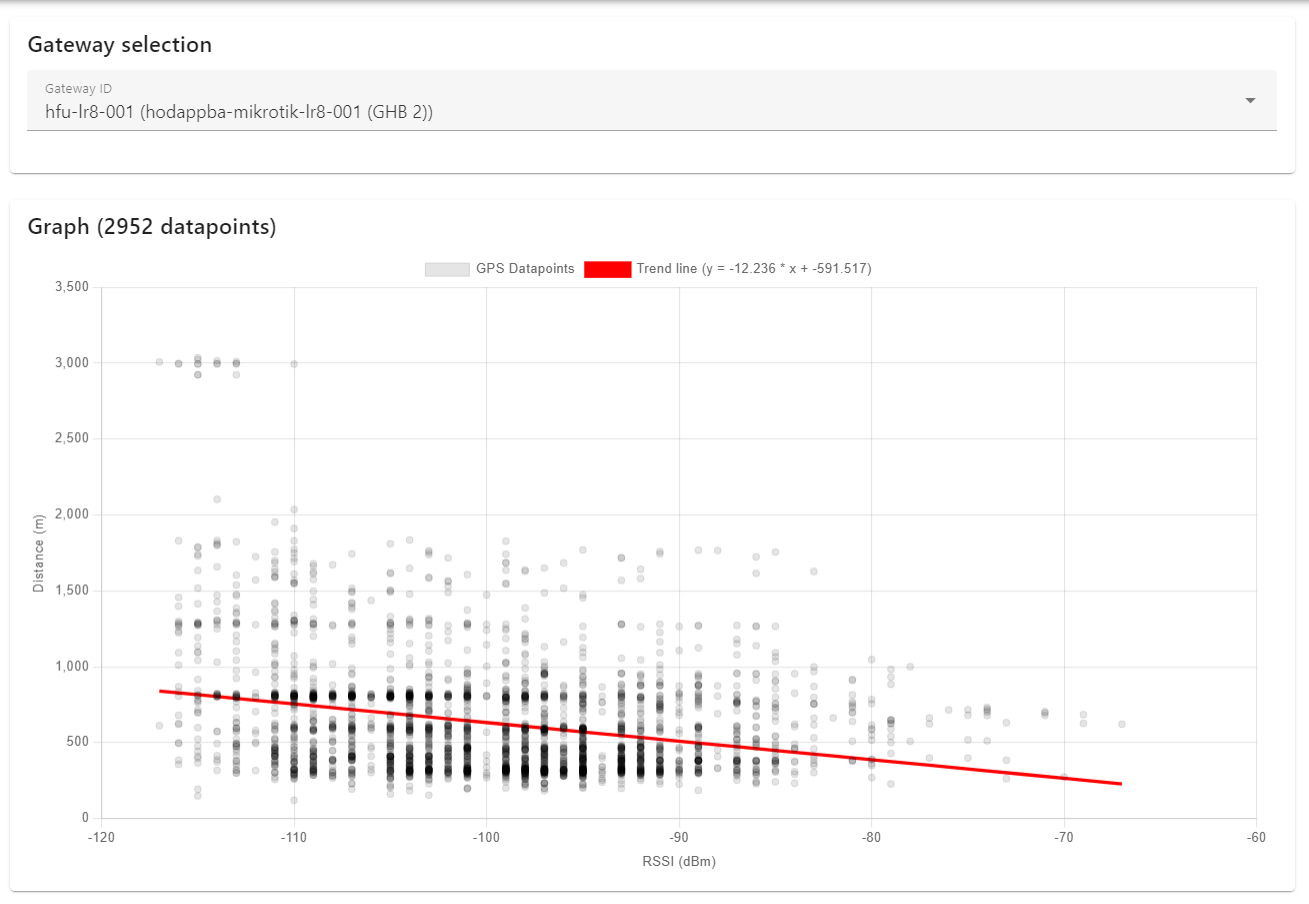
\includegraphics[width=1\textwidth]{pictures/ttn-locator/frontend/data/gateway_ghb_rssi_range_graph.png}
    \caption{Positive example of a \ac{RSSI} to distance graph the frontend of \ac{TTNL} can generate from data in its \ac{DB}\label{fig:rssi-range-graph-example}}
\end{figure}

\Cref{fig:rssi-range-graph-example} shows an example of a \ac{RSSI} to distance graph that the frontend of \ac{TTNL} generated.
It uses the \ac{RSSI} values of the device-based datapoints from a single gateway to generate the graph by calculating the distance to said gateway.
This makes it possible to determine the values of a linear regression function that can be used to calculate the distance to a gateway from a given \ac{RSSI} value.
Compared to the fixed \ac{RSSI} to range scale described in \cref{sec:fixed-rssi-to-range-scale}, this approach has the advantage that it can be used to generate a more accurate \ac{RSSI} to range scale by considering each gateway's behavior individually.

% TODO can this be said like this? outliers still seem kinda bad
While there are blatant outliers in the data, the graph still shows an average linear correlation between the \ac{RSSI} values and their distance.

\subsubsection{\ac{ToA}-based multilateration}

% TODO describe (with some data) why this didn't work (timestamps are not accurate enough and also sometimes way off)

One of the seemingly most promising techniques for locating \ac{LoRaWAN} nodes is \ac{ToA}-based multilateration.
As has been explained in \cref{sec:toa-based-multilateration}, this technique uses the time of arrival of a \ac{LoRa} signal to multiple gateways to calculate the position of the device that sent the signal using the speed of light.

Unfortunately, this technique did not work as expected in the scope of this thesis.
This was because the timestamps of signal arrival in the gateways that were used for this thesis were not accurate enough.
Differences of up to 1 second between the timestamps of the same signal in different gateways were not uncommon, making distance calculations using these values utterly unusable.

% TODO maybe take a better picture of this
\begin{figure}
    \centering
    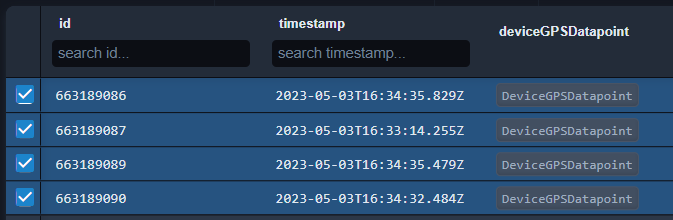
\includegraphics[width=0.6\textwidth]{pictures/multilateration/toa_bad_data_example_prisma_studio.png}
    \caption{Example of divergent timestamp data planned to be used for \ac{ToA} multilateration. The time difference between the first and second signal arrival amounts to more than one second. Picture taken from Prisma's \emph{Prisma Studio} web frontend.\label{fig:toa-bad-data-example}}
\end{figure}

\Cref{fig:toa-bad-data-example} shows an example of the divergent timestamp data that was planned to be used for \ac{ToA} multilateration where the time difference between the first and second signal arrival amounts to more than one second.
Since the speed of light is $299792458\ \mathrm{m/s}$, a difference of one second in the timestamps of two signals would result in a distance difference of $299792458\ \mathrm{m}$.
This is a distance that is too big to be useful for performing any sort of meaningful multilateration.

% TODO explain why this is the case and maybe how it could be fixed (using GPS time sync)

\subsubsection{Fingerprinting with \ac{RSSI} values}

% Show how this worked (quite alright, but needs a lot of pre-existing data)